\section{Mechanika tlakové desky}
\label{E4-mech_tlakovky}

Indukčně snímaná tlaková deska funguje díky čtyřem cívkám na desce ploš\-ných spojů, které mění svojí indukčnost podle vzdálenosti snímané desky, terčíku.
Z tohoto důvodu se terčík při používání naklání, čímž zároveň mění svojí vzdálenost od jednotlivých cívek. Z toho také plyne nutnost uložit terčík
částečně volně. Terčík je proto od snímací desky oddělen pružnou vložkou, která je zároveň předepnuta pomocí nažehlovací fólie, která kryje přední 
stranu dveří a spojuje terčík s čelní krycí deskou. Díky nažehlovací fólii je také přední část dveří voděodolná.

\begin{figure}[h]
    \centering
    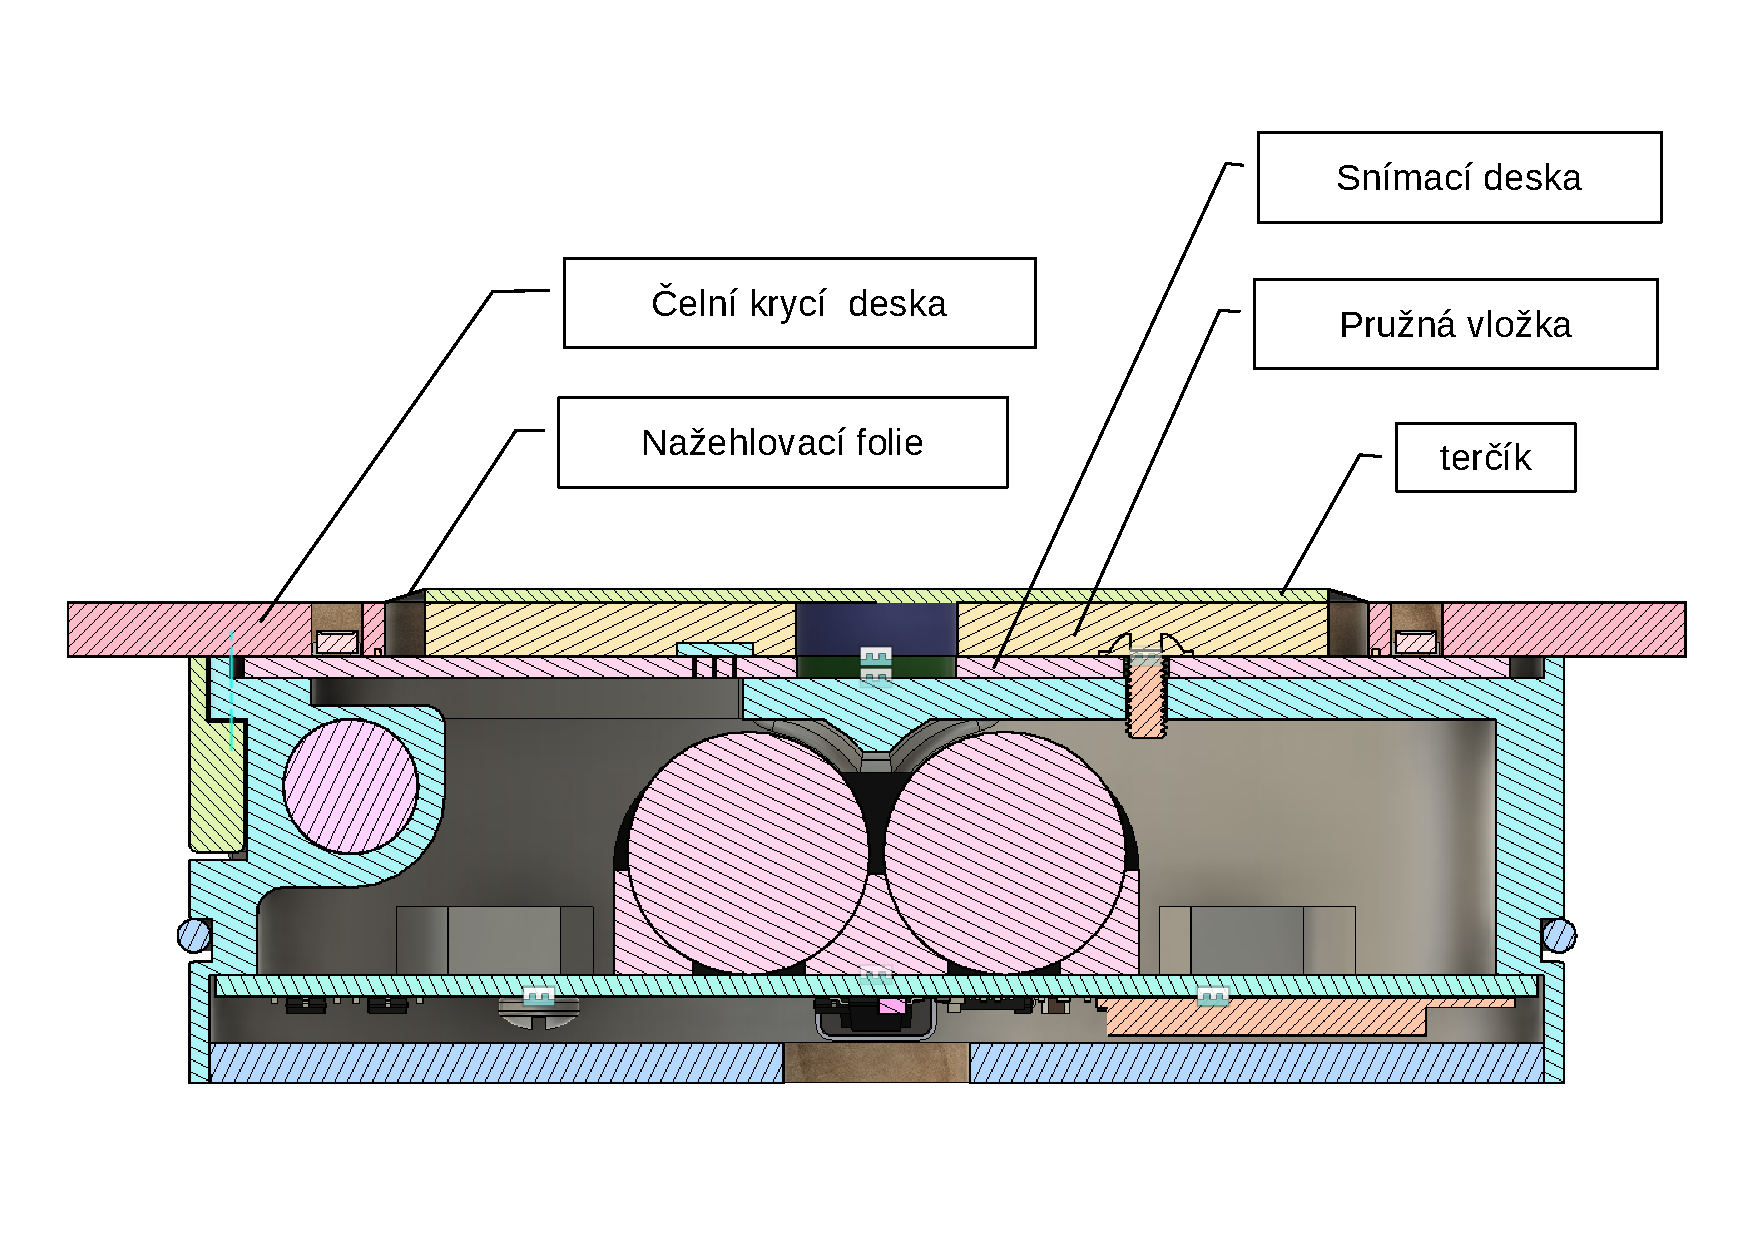
\includegraphics[width=\textwidth]{kapitoly/obrazky/E4/machanika_tlakove_desky/rez_po_ose.pdf}
    \caption{Řez varianty E4}
    \label{fig:E4-rez}
\end{figure}

Díky zkušenostem z jiného podobného projektu jsem zjistil, že ovládací prvek by měl být co možná největší. 
Zároveň by měl odolat i poměrně silným ranám, které děti v zápalu hry zařízení uštědřují.
Tlaková deska tedy počítá s možností působení síly o velikosti až 500~N, což samozřejmě zároveň znamená, že tělo dveří tomuto zatížení musí odolat.
Vzhledem k tomu, že nemám možnost vyrobit tělo z kovu a jsem odkázán na 3D tisk a laserovou řezačku, a zároveň chci mít dveře co možná nejmenší,
musel jsem napočítat kritické části těla tak, aby odolaly a zároveň nebyly příliš mohutné. Z tohoto důvodu jsem v programu Fusion 360, ve kterém jsem trezor vyvíjel,
dělal simulaci, kterou k práci přikládám na obrázcích \obr{fig:E4-simulace_tela} a \obr{fig:E4-simulace_tlakovky}.

Jako materiál těla jsem v první fázi zvolil standardní fotopolymer pro tiskárny typu SLA, s pevností v tahu 46 až 67 MPa.
V budoucnu bych ale chtěl tělo odlévat z nějakého houževnatého polyuretanu, aby se zlevnila výroba a zároveň stoupla odolnost.

